\documentclass[11pt]{article}
%	options include 12pt or 11pt or 10pt
%	classes include article, report, book, letter, thesis

\usepackage{amsmath}
\usepackage{array}
\setlength\extrarowheight{2pt}
\usepackage{graphicx}
\graphicspath{ {/home/shanedrafahl/coms331/hw0} }

\title{HW0}
\author{Shane Drafahl}
\date{23 August,2017}

\begin{document}
\maketitle

\fbox{\parbox{\dimexpr\linewidth-2\fboxsep-2\fboxrule\relax}{
 This is an inline equation $x + y = 3$  \\
 This is a displayed equation: \\
 \large \centerline{ $ x + \dfrac{y}{z - \sqrt{3}} = 2 $} \\
 This is how you define a piece-wise linear function: \\
 $$
f(x) = \left\{
        \begin{array}{ll}
        3x + 2 & $if x $<$ 0$ \\
        7x + 2 & $if x $ \geq $ 0 and x $<$ 10$ \\
        5x + 22 & $otherwise.$ \\
        \end{array}
    \right.
$$ \\

This is a matrix:
    \begin{center}
    \begin{tabular}{ |l|l|l|l| }

    \hline
    9 & 9 & 9 & 9 \\ [0.5ex]
    \hline
    6 & 6 & 6 &  \\ [0.5ex]
    \hline
    3 &  & 3 & 3 \\ [0.5ex]
    \hline
    \end{tabular}
    \end{center}

    This is a figure incorporated in a LaTeX file \\
    \\
    \centerline{ 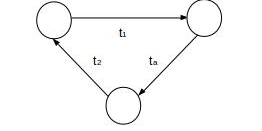
\includegraphics{graph.jpg} }
}}

$\newline$
2. Show that N (natural numbers) and Z (integer numbers) are equinumerous.
$\newline$
To show that the set of natural numbers and integer numbers are equinumerous
we have to show the cardinality of N and Z are the same. If there is a function
f: N $\rightarrow$ Z that is bijective then the cardinalities of sets N and Z would
be the same.
\newline

Suppose we have a function where $x \in N$ and $f(x) \in Z$

$$
f(x) = \left\{
        \begin{array}{ll}
        0 & $if x equals 0$ \\
        \frac{x}{2} * -1 & $if x mod 2 = 0$ \\
        \frac{(x - 1)}{2} + 1 & $otherwise.$ \\
        \end{array}
    \right.
$$ 

If f is onto then $\forall_{y} \in $ Z $ \exists_{x} \in N $ where $ f(x) = y $.
Using existential instantiation and universal instantiation either
$\frac{x}{2} * -1 = y$ or $\frac{(x - 1)}{2} + 1 = y$. If $ \frac{x}{2} * -1 = y $.
For $\frac{x}{2} * -1 = y$ is equal to x = -2y and $\frac{(x - 1)}{2} + 1 = y$ equals
2y - 1 = x. If y is negative then for -2y = x, x will equal a natural number. If y is positive
then 2y - 1 = x, x will equal a natural number because it cannot be negative and y cant be 0 because
x will be 0 as well. So therefore for all values of y a natural number of x can be reached so therefor
function f is onto.
$\newline \newline$
Using proof by contradiction assume f is not one to one so $\exists_{x}\exists_{y}(f(x) = f(y)
\rightarrow x \neq y \land x, y \in N \land x, y)$. If x is odd and y is even or vice versa then
$\frac{y}{2} * -1 = \frac{(x - 1)}{2} + 1 $. This can be reduced to y = -x - 1. This is a contradiction
because since x and y are natural numbers they cannot be negative so $ 0 > -x - 1 $ and $ y > 0 $ so therefore
they cannot be equal. If x and y are both even then $ \frac{y}{-2} = \frac{x}{-2} $ which reduces to
x = y which is a contradiction because x and y cannot equal each other. If x and y are both odd then
$ \frac{(y - 1)}{2} + 1 $ = $ \frac{(x - 1)}{2} + 1 $ which reduces down to x = y and for the same
reason is a contradiction because x and y equal each other.
$\newline \newline$
therefore the function f is one to one and onto so it is bijunction and therefore natural
numbers have the same cardinality as integers and are are equinumerous.
$ \newline \newline$
3. Let f : S $ \rightarrow $ S  be a total function. Prove that, if S is infinite, f can be one-to-one without
being onto, and onto without being one-to-one.
$\newline \newline$
For f to be one-to-one but not onto for f(x) = y where $x \in S $ and $ y \in S $ there is at least one value
of y and x $ f(x) \neq y $.

$$
f(x) = \left\{
        \begin{array}{ll}
        x + 1 & $ if x $ \geq $ 0 $ \\
        x - 1 & $otherwise.$ \\
        \end{array}
    \right.
$$ \\

$ \newline $
Function f cannot be 0. If x is greater or equal to 0 then 0 = x + 1. The only value for x where this could be
true is x = -1 but x cannot be a negative number. Otherwise for 0 = x - 1 x would need to be equal to 1
but x cannot equal or greater than 0 so therefore for either case 0 is an element of S but $ f(x) \neq 0 $.
$ \newline \newline $
To prove that f is one to one we will use proof by contradiction and assume that function f is not
one to one so there is some value $ \exists_{x} \exists_{y} \in S $ where $ x \neq y \land f(x) = f(y) $
so if x is equal to 0 or greater and y is less than 0 or vice versa so x + 1 = y - 1 which can be reduced to
x + 2 = y. This is a contradiction because y in this case is less than 0 and x can either be 0 or greater so
adding 2 to 0 or greater cannot result in a negative number. If x and y are greater or equal to 0 then
x + 1 = y + 1 or if they are both less than 0 so x - 1 = y - 1 but these both can be reduced to x = y
and this is a contradiction because $ x \neq y $ so therefore the function f is one to one.
$ \newline \newline $
A function f can be onto and not one-to-one
$ \newline \newline $
$ x \in S \newline $

$$
f(x) = \left\{
        \begin{array}{ll}
        0 & if $ x = 0 $ \\
        x + 1 & if $ x $ < $ 0 $ \\
        x - 1 & if $ x $ > $ 0 $ \\
        \end{array}
    \right.
$$ \\

$ \newline \newline $
f is is not one-to-one because f(0) = f(-1) = f(1) = 0. Function f is onto. If
x is greater than 0 then $ y \in S $ so y = x - 1. This can be reduced to 1 + y = x.
The value y can be any value in S and correspond to a value x which is also in S. Otherwise
if x is 0 y is 0 and if x is less than 0 then y = x + 1. This can be reduced to y - 1 = x. For any value
$ y \in S $ $ x \in S $ every value of y corresponds to a value x. Therefore the function f is onto.
$\newline \newline$
4. Show that the relation R defined by
    $\newline \newline$
    $\forall_{m,n} \in N, $ (m, n) $ \in R $ $ \Leftrightarrow $ (m - n) mod 3 = 0
    $\newline \newline$
    is an equivalence relation, and describe its equivalence classes.
    $\newline \newline$
    The relation R is reflexive because for any real number x, (x - x) mod 3 = 0 because x - x will always be 0.
    $\newline \newline$
    The relation R is symmetric because for any real numbers x and y this say x - y = z so y - x = -z. So by
    swapping the order of x and y the relation is z mod 3 = 0 or -z mod 3 = 0. If z is negative or not
    makes no difference for mod so therefore R is symmetric.
    $\newline \newline$
    The relation R is transitive. Suppose x,y,z are all real numbers. Suppose R(x, y) is true
    so (x - y) mod 3 = 0. R(y, z) is also true so (y - z) mod 3 = 0. Since we know that (x,y) is
    true we can assume that (x-y) = 3p or this can be reduced to x = 3p + y and the same for (y-z) = 3f
    which can be reduced to z = y - 3f. So for R(x, z) would be (3p + y) - (y - 3f) = 3f + 3p or 3(f + p).
    3(f + p) mod 3 will always be 0 so therefore it is true and relation R is transitive.
    $\newline \newline$
    Relation R is reflexive, symmetric, and transitive so therefore is a equivalence relation.
    The equivalence class for this relation R $ [x]_{R} =  \{\ y \mid (x, y) \in R \}\ $ where y is equal to any multiple of 3.
$\newline \newline$
5. Show that $ \sum\limits_{i=1}^n i^2 $ = (2n + 1)(n + 1)n/6
$\newline \newline$
Using weak induction on the natural number
$\newline \newline$
Basis: $ \sum\limits_{i=1}^1 i^2 $ = 1 and (2 + 1)(1 + 1)1/6 = 1
$\newline \newline$
Inductive Hypothesis: For $ \sum\limits_{i=1}^n i^2 $ is equal to (2n + 1)(n + 1)n/6 and true
for n.
$\newline \newline$
Inductive Step: 
To prove for n+1 this get the n + 1. (2(n + 1) + 1)(n + 2)($\frac{n + 1}{6}$). This reduces 
to $\frac{2n^{3} + 7n^{2} + 6n}{6} + \frac{2n^{2} + 7n + 6}{6} = \frac{2n^{3} + 9n^{2} + 13n + 6}{6}$.
Now we will find $ \sum\limits_{i=1}^{n + 1} i^2 $ = (2n + 1)(n + 1)$\frac{n}{6}$ + $(n + 1)^{2}$ this
reduces to $\frac{(2n^{3} + 3n^{2} + n)}{6}$ + $\frac{(6n^{2} + 12n + 6)}{6}$ = $\frac{2n^{3} + 9n^{2} + 13n + 6}{6}$.
So therefore n + 1 is correct. 



\end{document}
